% Tesis UNADE CLASS -- version 0.1
% Clase para las tesis del UNADE
% 
% 2025 09 02 Carlos Urteaga carlos(dot)urteaga (at) outlook (dot) com
% LICENSE: Creative Commons SA-BY 3.0
% Este documento presenta un ejemplo de uso de la plantilla
% El estudiante es libre de modificar este archivo a su gusto

\documentclass{tesisUNADE}

\usepackage[utf8]{inputenc}
\usepackage{type1cm,lettrine}
\usepackage{longtable}
 \usepackage{eso-pic}
 \usepackage{xcolor}
 \usepackage[margin=1in]{geometry} % left margin defines where the stripe will sit
 \usepackage{lipsum}
\usepackage[toc,style=altlistgroup,hyperfirst=false]{glossaries}
\usepackage{lscape}
\usepackage{subcaption}
\usepackage{float}
\usepackage{amsopn}


\usetikzlibrary{babel}

% Glossary
\newcommand\nomenclature[2]{#1 & #2 \\}

\title{Nombre del Proyecto}
\degree{Nombre del Programa}
\author{Nombre}
\renewcommand{\student}{Alumno} %change the value to Alumne if is desired

% \setadvisorlabel{Directora}     % o "Director(a)"
% \setcoadvisorlabel{Codirectora} % o "Co-Director(a)"
\advisor{Nombre del Director}
%\coadvisor{Nombre del Codirector}
\year{2025}


\definecolor{myyellow}{RGB}{255,204,0}
\definecolor{myblue}{RGB}{0,51,153}

%%%%%%%%
\begin{document}

\pagenumbering{gobble}
\maketitle

\begin{abstract}{spanish}
\lipsum[1]

\end{abstract}
Palabras clave: Entre 3 y 5 palabras. No poner en cursiva. 
\begin{abstract}{english}
\lipsum[1]
\end{abstract}
Keywords: 

%%%%%%%%%%%%%%%%%%%%%%%%%%%%%%%%%%%%%%%%%%%%%%
% ABSTRACT
%%%%%%%%%%%%%%%%%%%%%%%%%%%%%%%%%%%%%%%%%%%%%%

\vspace*{3cm}

\thispagestyle{empty}
\begin{center}
   \hfill \emph{Lorem ipsum dolor sit amet, \\\hfill consectetur adipiscing elit. \\\hfill Sed do eiusmod tempor incididunt \\\hfill ut labore et dolore magna aliqua.\\
   \vspace*{2cm}\hfill
   Lorem ipsum dolor sit amet, \\\hfill consectetur adipiscing elit. \\\hfill Sed do eiusmod tempor incididunt \\\hfill ut labore et dolore magna aliqua.\\
   \vspace*{2cm}\hfill
   Lorem ipsum dolor sit amet, \\\hfill consectetur adipiscing elit. \\\hfill Sed do eiusmod tempor incididunt \\\hfill ut labore et dolore magna aliqua.\\
\vspace*{2cm}\hfill
Lorem ipsum dolor sit amet, \\\hfill consectetur adipiscing elit. \\\hfill Sed do eiusmod tempor incididunt \\\hfill ut labore et dolore magna aliqua.\\}
\end{center}
\chapter*{Agradecimientos}
Lorem ipsum dolor sit amet, consectetur adipiscing elit. Sed do eiusmod tempor incididunt ut labore et dolore magna aliqua.


Lorem ipsum dolor sit amet, consectetur adipiscing elit. Sed do eiusmod tempor incididunt ut labore et dolore magna aliqua.


Lorem ipsum dolor sit amet, consectetur adipiscing elit. Sed do eiusmod tempor incididunt ut labore et dolore magna aliqua.


\selectlanguage{spanish}

\pagenumbering{roman}
\renewcommand{\contentsname}{Tabla de contenido}
\tableofcontents
\setcounter{page}{1}
\renewcommand{\listfigurename}{Tabla de figuras}
\renewcommand{\listtablename}{Tabla de tablas}
\listoftables
\listoffigures

%%%%%%%%%%%%%%%%%%%%%%%%%%%%%%%%%%%%%%%%%%%%%%
% Document  
%%%%%%%%%%%%%%%%%%%%%%%%%%%%%%%%%%%%%%%%%%%%%%


\chapter*{Lista de Acrónimos}
\begin{longtable}{@{}p{3cm}@{}p{\dimexpr\textwidth-1cm\relax}@{}}


\nomenclature{\textbf{UNADE}}			{Universidad Americana de Europa}

\end{longtable}

\newpage
\pagenumbering{arabic}
\setcounter{page}{1}

%%%%%%%%%%%%%%%%%%%%%%%%%%%%%%%%%%%%%%%%%%%%%%
% CONTENT  
%%%%%%%%%%%%%%%%%%%%%%%%%%%%%%%%%%%%%%%%%%%%%%

 \chapter{Introducción}\label{Cap_00}

\section{Descripción del problema}
Descripción de la problemática que resolverá la tesis, explicando la relevancia de poder resolverla, como surge, cuál es el motivo para resolverla, a quien beneficiará si se resuelve y demás aspectos concernientes al problema a resolver.

\section{Hipótesis}
Debe ser un enunciado de máximo un párrafo en donde debes escribirse con la siguiente estructura:
La primera parte es la descripción afirmativa de lo que hará tu tesis y finalmente lo que se conseguirá como resultado de aplicarla. Ejemplo: “Si diseño una metodología de implementación de una red segura con diversas técnicas de cifrado, mejoraré la seguridad integral de las empresas que la implementen”.

\section{Justificación}
Son los motivos por los cuales es viable el desarrollo de la tesis, ¿Por qué es relevante que se resuelva este problema?, ¿Que viabilidad tiene, en cuanto a implementación, realización, costo-beneficio, esfuerzo, etc.?, ¿A quién beneficiará? ¿Que aportará?, ¿Tendrá un costo menor de algo similar en el mercado?, ¿Realizará algo mejor que otro desarrollo similar?, etc.

\section{Objetivos}
Objetivo general. Se detalla de forma general que va a realizar el trabajo de tesis.
Objetivos específicos. Es el conjunto de objetivos intermedios que permitirán completar el objetivo general, por lo general se enlistan en orden cronológico y debe ser medible.

\section{Organización del documento de tesis}
Se detallan el contenido de los capítulos siguientes.
\chapter{Marco de referencia}\label{Cap_00}
\lettrine[lines=2,nindent=0pt]{E}{}l presente capítulo muestra un contexto de la inteligencia artificial y su impacto en el sector financiero. También se presenta el objetivo, alcance y metodología utilizada en este trabajo. Al final del capítulo se detalla la organización del documento.

\section{Marco Teórico}
Aproximadamente de 20 a 40 cuartillas. Son todos los temas que se deben de saber para comprender el desarrollo de la tesis, Ejemplo: SI la tesis es referente a “un algoritmo de Inteligencia artificial para la elaboración de nano robots que construyan computadoras cuánticas”, en el marco teórico debe de venir la teoría referente a: Algoritmos de inteligencia artificial, elaboración de nano robots y construcción de computadoras cuánticas.

\section{Estado del arte}
Aproximadamente de 20 a 40 cuartillas. En este apartado se investigan todos los desarrollos similares a la tesis que estas realizando, primero en tu país de origen y posteriormente en el mundo, la aportación de este apartado es darse cuenta si lo que estamos haciendo es algo que está desarrollando en nuestro país o en el mundo, que tan viable es, que tan original es, que tanto diferente estoy aportando, etc.

\chapter{Metodología, Diseño, Software o Implementación propuesta}\label{Cap_02}
\lettrine[lines=2,nindent=0pt]{S}{}e debe explicar la metodología, diseño, software o implementación propuesta, donde se detalle lo siguiente:

\begin{itemize}
\item El problema que resolverá
\item Descripción general de la solución propuesta
\item Descripción detallada de cada fase, etapa, módulo, etc.
\item En esta sección se describe tu aportación de la tesis, por lo que es necesario conjuntar todo el conocimiento previo del marco teórico, estado del arte y metodologías estudiadas para que tu trabajo sea fundamentado, sustentado y factible de desarrollar o implementar.
\item Debe tener calidad argumentativa, es decir, que sea congruente con lo investigado hasta ahora, marco teórico y estado del arte.
item referencia a la figura (figure \ref{fig:figure})
\item Tabla \ref{table:1} es un ejemplo de un elemento en \LaTeX{}.

\end{itemize}

\begin{figure}[H]
    \begin{center}
    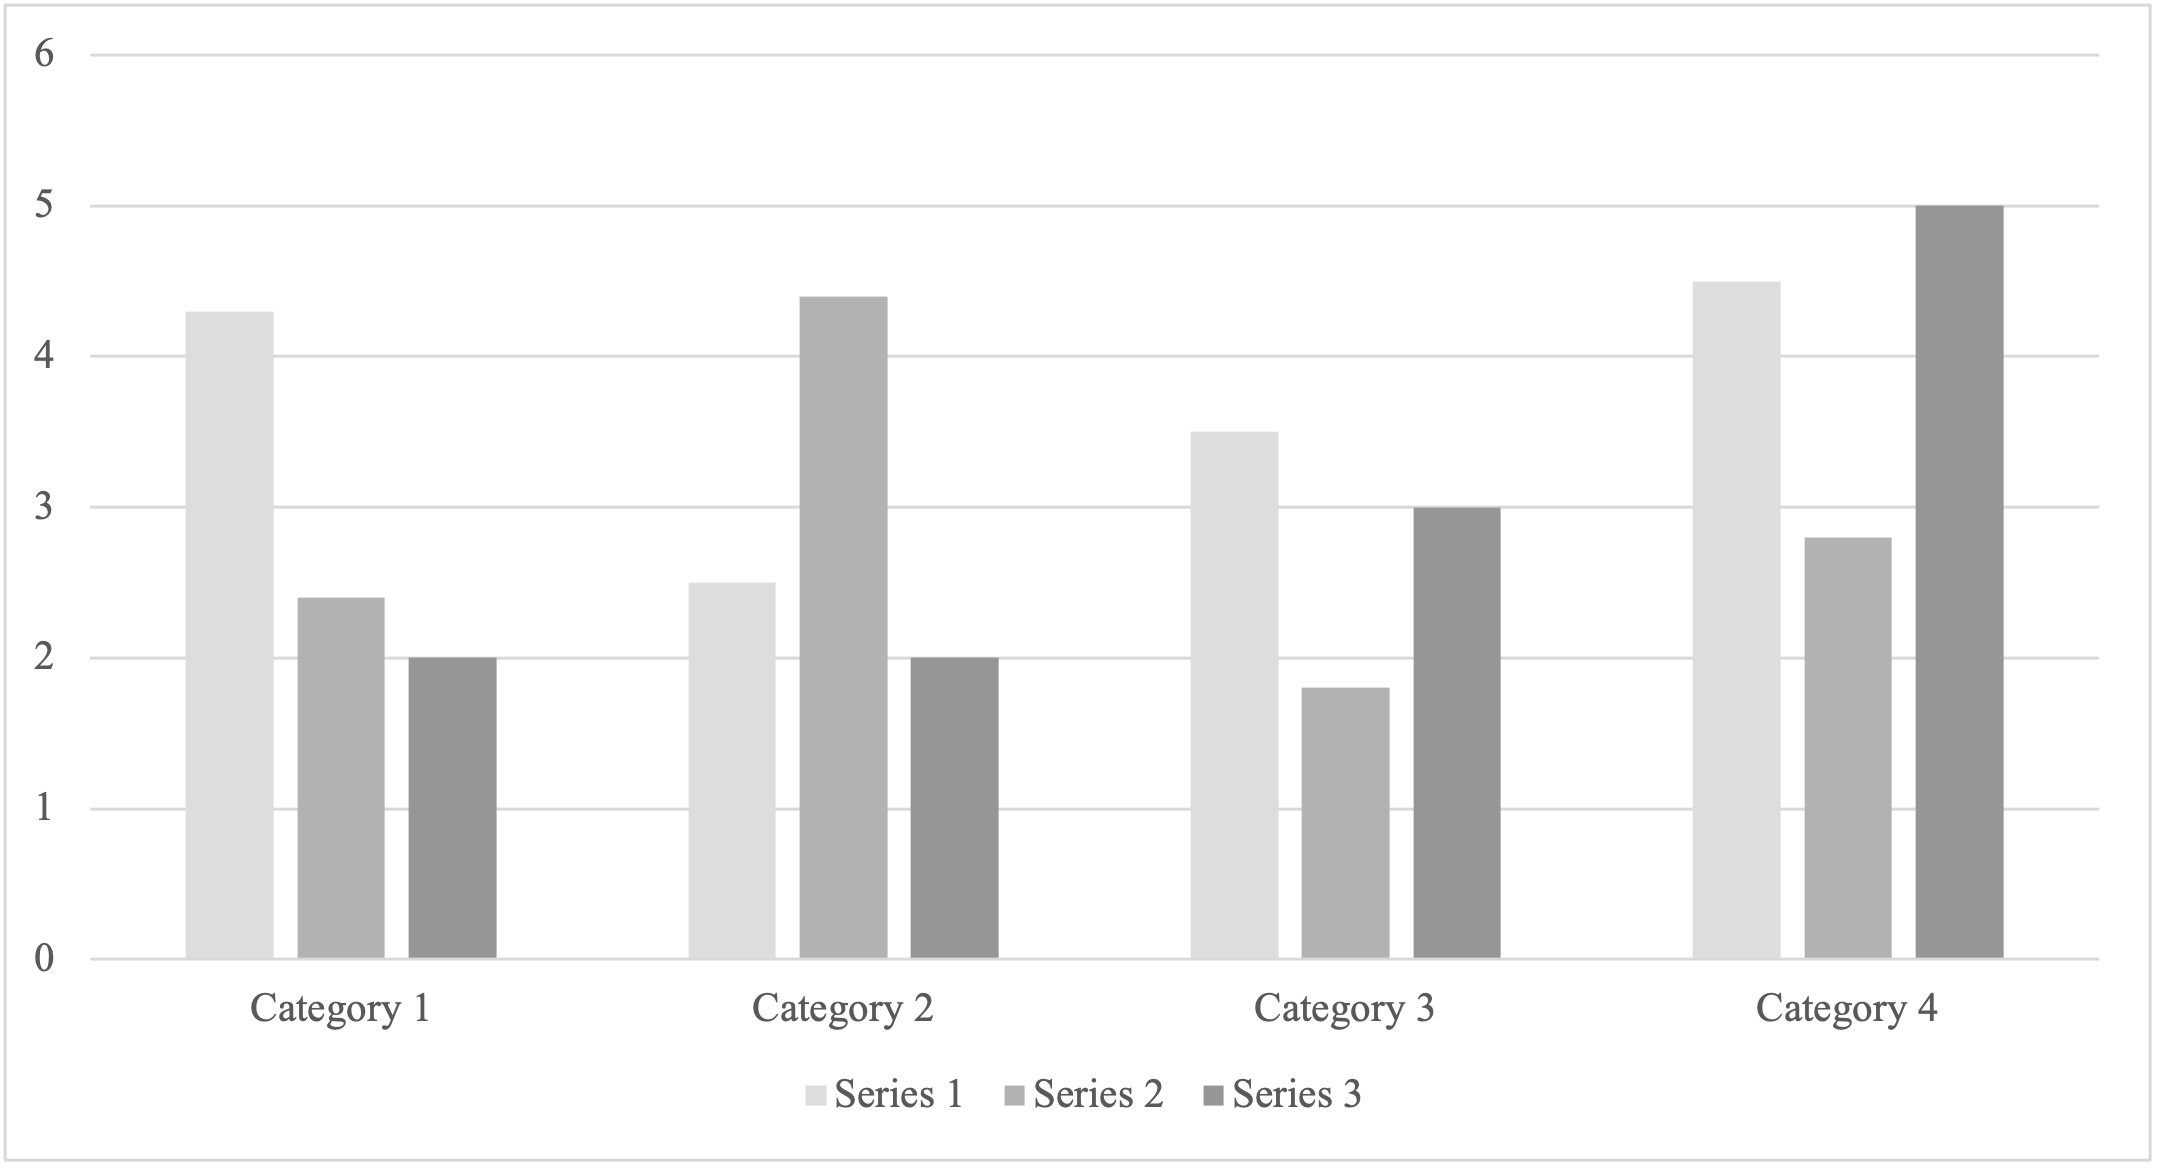
\includegraphics[width=.8\textwidth]{Cap_02/grafica.png}\caption[Metodología CRISP-DM]{Include all figures in their own section, following references (and footnotes and tables, if applicable).  Include a numbered caption for each figure.  Use the Table/Figure style for easy spacing between figure and caption.]}\label{fig:figure}
    \end{center}
    \end{figure}



    \begin{table}[h!]
    \centering
    \caption{Table to test captions and labels.}
    \label{table:1}
    \begin{tabular}{c c c c} 
     \hline
     Col1 & Col2 & Col2 & Col3 \\ [0.5ex] 
     \hline
     1 & 6 & 87837 & 787 \\ 
     2 & 7 & 78 & 5415 \\
     3 & 545 & 778 & 7507 \\
     4 & 545 & 18744 & 7560 \\
     5 & 88 & 788 & 6344 \\ [1ex] 
     \hline
    \end{tabular}
    \end{table}
\chapter{Pruebas y Resultados}\label{Cap_03}
\lettrine[lines=2,nindent=0pt]{E}{}n esta sección se muestran todas las pruebas realizadas, complicaciones, adecuaciones, hallazgos y resultados encontrados, lo cual va ligado con la hipótesis propuesta, la cual debe validarse en esta sección.
\chapter{Conclusiones}\label{Cap_04}
\lettrine[lines=2,nindent=0pt]{S}{}e redactan toda la información sobresaliente de tu tesis, de la metodología, de los hallazgos encontrados, de los resultados y sobre todo cuál es tu aportación principal realizada. 
\cite{unade2025}

%%%%%%%%%%%%%%%%%%%%%%%%%%%%%%%%%%%%%%%% %%%%%%
% BIBLIOGRAPHY
%%%%%%%%%%%%%%%%%%%%%%%%%%%%%%%%%%%%%%%%%%%%%%
\clearpage
%\renewcommand\bibname{Referencias Bibliográficas}
%\cleardoublepage  
%\markboth{\bibname}{\bibname}
\bibliography{bibtex}
\bibliographystyle{ieeetr}
\end{document}
